\begin{figure}[H]
\centering
	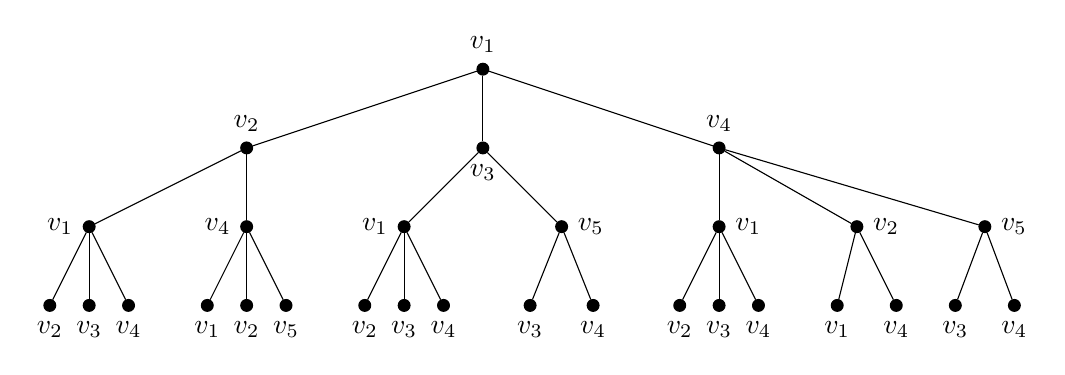
\begin{tikzpicture}

      \tikzset{enclosed/.style={draw, circle, inner sep=0pt, minimum size=.15cm, fill=black}}
%% Vertices
      	\node[enclosed, label={above: $v_1$}] (v1) at (3,6) {};
      	\node[enclosed, label={above: $v_2$}] (v2) at (0,5) {};
    		\node[enclosed, label={below: $v_3$}] (v3) at (3,5) {};
  	    \node[enclosed, label={above: $v_4$}] (v4) at (6,5) {};
     	\node[enclosed, label={left: $v_1$}] (v5) at (-2,4) {};
     	\node[enclosed, label={left: $v_4$}] (v6) at (0,4) {};
     	\node[enclosed, label={left: $v_1$}] (v7) at (2,4) {};
     	\node[enclosed, label={right: $v_5$}] (v8) at (4,4) {};
     	\node[enclosed, label={right: $v_1$}] (v9) at (6,4) {};
     	\node[enclosed, label={right: $v_2$}] (v10) at (7.75,4) {};
     	\node[enclosed, label={right: $v_5$}] (v11) at (9.375,4) {};
     	\node[enclosed, label={below: $v_2$}] (v12) at (-2.5,3) {};
      	\node[enclosed, label={below: $v_3$}] (v13) at (-2,3) {};
  	    \node[enclosed, label={below: $v_4$}] (v14) at (-1.5,3) {};
  	    \node[enclosed, label={below: $v_1$}] (v15) at (-0.5,3) {};
     	\node[enclosed, label={below: $v_2$}] (v16) at (0,3) {};
     	\node[enclosed, label={below: $v_5$}] (v17) at (0.5,3) {};
     	\node[enclosed, label={below: $v_2$}] (v18) at (1.5,3) {};
      	\node[enclosed, label={below: $v_3$}] (v19) at (2,3) {};
  	    \node[enclosed, label={below: $v_4$}] (v20) at (2.5,3) {};
  	    \node[enclosed, label={below: $v_3$}] (v21) at (3.6,3) {};
  	    \node[enclosed, label={below: $v_4$}] (v22) at (4.4,3) {};
  	    \node[enclosed, label={below: $v_2$}] (v23) at (5.5,3) {};
      	\node[enclosed, label={below: $v_3$}] (v24) at (6,3) {};
  	    \node[enclosed, label={below: $v_4$}] (v25) at (6.5,3) {};
  	    \node[enclosed, label={below: $v_1$}] (v26) at (7.5,3) {};
     	\node[enclosed, label={below: $v_4$}] (v27) at (8.25,3) {};
     	\node[enclosed, label={below: $v_3$}] (v28) at (9,3) {};
     	\node[enclosed, label={below: $v_4$}] (v29) at (9.75,3) {};
%Edges
		\path (v1) edge node[midway, sloped, above] {} (v2);
		\path (v1) edge node[midway, sloped, above] {} (v3);
		\path (v1) edge node[midway, above] {} (v4);
		\path (v2) edge node[near end, sloped, below] {} (v5);
		\path (v2) edge node[midway, below] {} (v6);
		\path (v3) edge node[near end, sloped, above] {} (v7);
		\path (v3) edge node[near end, sloped, above] {} (v8);
		\path (v4) edge node[near end, sloped, above] {} (v9);
		\path (v4) edge node[near end, sloped, above] {} (v10);
		\path (v4) edge node[near end, sloped, above] {} (v11);
		\path (v5) edge node[near end, sloped, above] {} (v12);
		\path (v5) edge node[near end, sloped, above] {} (v13);
		\path (v5) edge node[near end, sloped, above] {} (v14);
		\path (v6) edge node[near end, sloped, above] {} (v15);
		\path (v6) edge node[near end, sloped, above] {} (v16);
		\path (v6) edge node[near end, sloped, above] {} (v17);
		\path (v7) edge node[near end, sloped, above] {} (v18);
		\path (v7) edge node[near end, sloped, above] {} (v19);
		\path (v7) edge node[near end, sloped, above] {} (v20);
		\path (v8) edge node[near end, sloped, above] {} (v21);
		\path (v8) edge node[near end, sloped, above] {} (v22);
		\path (v9) edge node[near end, sloped, above] {} (v23);
		\path (v9) edge node[near end, sloped, above] {} (v24);
		\path (v9) edge node[near end, sloped, above] {} (v25);
		\path (v10) edge node[near end, sloped, above] {} (v26);
		\path (v10) edge node[near end, sloped, above] {} (v27);
		\path (v11) edge node[near end, sloped, above] {} (v28);
		\path (v11) edge node[near end, sloped, above] {} (v29);

	\end{tikzpicture}
	\caption{De mulige løsninger for veje med længde 3 fra $v_{0}$ til $v_{k}$.}
	\label{fig.vaegtetopg}
\end{figure}